\documentclass[12pt,a4paper]{report}


\usepackage{pgfplotstable}
\usepackage{pgfplots}



%\usepackage{tocloft}

%glossar
%\usepackage[xindy]{glossaries}

% Bibliography Quellen.
% Immer nur eine verwenden
%\usepackage{natbib} % Zitate mit Namen + Jahr
\usepackage{cite} % Zitate mit Nummern

% Eigene Style-Datei mit weiteres Includes
\usepackage{projekt}

% Pakete f�r Links
\usepackage{hyperref}
\usepackage{url}

\usepackage{glossaries}
\makeglossaries


\author{Dennis Sebastian Rieber}
\title{Research Project Report}
\setTopic{Extension of CUDA's unified memory API with NUMA aware features}
\setFackultaet{Department of Physics and Astronomy}
\setBetrieb{University of Heidelberg}
\setInstitute{ZITI, Chair of Application Specific Computing}
\setSupervisor{Prof. Dr. Robert Strzodka}
\setStudiengang{Computer Engineering}

\begin{document}
% Set Font (If we don't want times)
%\changefont{phv}{m}{n} % (SansSerif) Helvetica
%\changefont{ppl}{m}{n} % Palantino
%\changefont{pnc}{m}{n} % New Century Schoolbook

% preface with roman numbers
\maketitle
\newpage % Newpage required for correct pagination

% Roman counting for ToC
\setcounter{page}{1}
\pagenumbering{Roman}

\begin{abstract}
NUMA effects can have a big influence on an application's performance, yet many frameworks like CUDA pay no attention
to NUMA locality. This project shows how CUDA applications can be made NUMA aware with a minimally invasive wrapper
API and explores how this may impact application performance. The results show that correct NUMA placement between
device and host can lead to an increase in overall performance, which is impaired by an overly expensive allocation process.
\end{abstract}

\tableofcontents
\newpage % Newpage required for correct pagination

% 1.5 linespacinfg
\singlespacing
%\onehalfspacing

\clubpenalty = 10000 % schliesst Schusterjungen aus 
\widowpenalty = 10000 \displaywidowpenalty = 10000% schliesst Hurenkinder aus

% Equation listing
\newcommand{\listequationsname}{Gleichungsverzeichnis}
%\newlistof{myequations}{equ}{\listequationsname}
\newcommand{\myequations}[1]{%
\addcontentsline{equ}{myequations}{\protect\numberline{\theequation}#1}\par}

	%\include{praeamble}
	% Document with regular arabic pagination
	\pagenumbering{arabic}
	\setcounter{page}{1}
	\chapter{Introduction}\label{c:moti}
\begin{figure}[b!]
	\begin{center}
	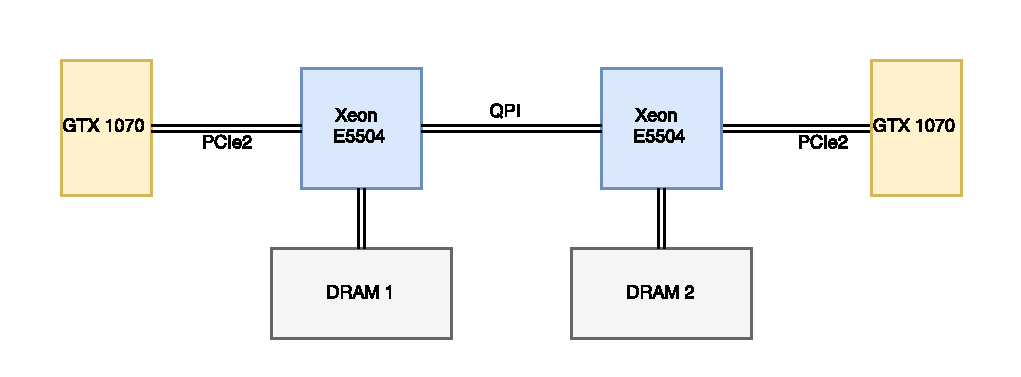
\includegraphics[width=.75\textwidth]{system}
	\label{f:sys}
	\caption{Test system, as described in chapter \ref{c:eval}. The QPI-Link between the two CPUs is the NUMA domain border.}
	\end{center}
\end{figure}
For Non-Uniform Memory Access(NUMA) architectures, research has shown that handling physical data locality has a positive influence on performance, yet few libraries and framework offer tools for fine-grained 
management of data locality. 
While in NVidia's CUDA framework device memory can be managed on a rather fine scale, host memory is treated as a single location, ignoring the possibility of underlying NUMA architectures.

In a system with multiple  NUMA-nodes, GPUs are either evenly distributed between all nodes or clustered on one or a few nodes. This connection to a node is the result of the PCIe controller that is part
	of the CPUs package. Regardless on how the system is configured, there are certain NUMA nodes, thus certain physical memory regions that are closer to one GPU than to a GPU that is connected to a different PCIe controller. Placing data on a NUMA node not directly connected to the GPU device causes lower host/device bandwidth due to indirection via HT/QPI for each memory access. An example for such a system is displayed in Figure \ref{f:sys}.

This project presents a way to explicitly set the NUMA-affinity for data allocations and movements with CUDA's unified memory. Chapter \ref{c:target} defines the goals of the project, and the means to reach them. Chapter \ref{c:env} presents the memory technologies and how they can be used and manipulated. Chapter \ref{c:impl} shows how these technologies are combined to achieve the defined goal. The resulting wrapper and the performance are evaluated in chapter \ref{c:eval}.


	\chapter{Project Goals}\label{c:target}
The goal of this project is to explore the possibilities of extending CUDA's unified memory (UM) functions to 
NUMA nodes and represent them in the same way a CUDA device is represented, with regards to data-movement
of an application. This project evaluates if and how the tools that manipulate NUMA affinity of memory pages can be applied to imitate the behaviour of CUDA's unified memory on the host side. The goal is to enable placement of
host-side data close to the used CUDA devices in order to minimize latency and maximize bandwidth.

An evaluation of the available tools for NUMA manipulation is performed in order to determine which tool
should be used in the implementation. Differences in performance and memory footprint are reviewed.
Because unified memory requires an allocation via the CUDA Runtime API, this project reviews how data
is allocated by CUDA and the possibilities of manipulating affinity.

The extension of CUDA's UM functionalities is implemented as a wrapper with a minimally invasive API. By using
function signatures that allow a simple search and replace operation in existing code, every application
can be made NUMA aware with little effort.
The resulting API wrapper is used to evaluate the NUMA affinity in CPU/GPU heterogeneous applications in
order to determine if and when it is beneficial and which factors are contributing to this.
%
%\begin{itemize}
%	\item Extending of CUDAs UM behavior to NUMA Nodes by:
%	\item Evaluation of Unified Memory abilities
%	\item Evaluation of Linux Memory abilities
%	\item Replication of UM behavoir for numa nodes with a minimal invasive API
%	\item Performance Evaluation
%\end{itemize}
	\chapter{Memory Management Resources}\label{c:env}
%\begin{itemize}
%	\item Linux Memory
%	\item --Virtual and Physical Memory in NUMA Systems
%	\item --Hardware Locality (hwloc)
%	\item --Post Allocation Memory Migration
%	\item CUDA Memory
%	\item -- Unified Memory
%\end{itemize}
The following chapter introduces the reader to the memory management systems
utilized in this project and how they work, in order to impart the knowledge required
to understand the decision made during the project. The following sections will 
discuss how memory is managed and represented in the operating system (Linux) and how NVidias CUDA framework is handling memory, both on host and device side. The focus is on
how memory pages can be allocated and migrated between physical memory locations inside a NUMA systems.

\section{Virtual and Physical Memory in NUMA Systems}\label{sec:vpm}
The virtual memory hides the tasks of memory allocation and access in a NUMA architecture from the user, but allows
users to manipulate the default behaviour for specific needs. 

By default, Linux uses lazy memory allocation. Memory allocated by a program has no physical representation before the memory page is written for the first time. Only then it will be assigned to a physical memory location (and thus a NUMA node). 
The NUMA node on which the thread is executed
which is the first to write a value to the memory page, is the node in which physical
memory the memory page is stored. This behaviour is called the "first touch" policy and
is intended to ensure NUMA locality.
Data that resides in physical memory that belongs
to a NUMA node can be access with a higher bandwidth and less latency than memory which is 
located on a remote node.

The physical location of a page is fixed and will not change by itself during its lifetime, even if the thread that created the data has migrated to another NUMA node. This behaviour can be an issue for memory bound computations, since their performance is likely to suffer under the reduced memory bandwidth. \cite{Linux:Memdoc}
\begin{figure}[hbtp]
	\begin{tikzpicture}
	\begin{axis}[
	width=\textwidth,
	height=8cm,
	xlabel={Sample Size (MB)},
	ylabel={Bandwidth (GB/s)},
	grid=major,
	legend entries={hwloc 1T, first touch1T, hwloc 8T, first touch 8T},
	% ymode=log,
	xmode = log,
	legend pos=north west,
	legend cell align=left
	]
	\addplot[thick,mark=o,blue,each nth point={8}] table[x index={0}, y index={2}] {../../../data/migrate_hwloc_o3.dat};
	\addplot[thick,mark=o,red,each nth point={8}] table[x index={0}, y index={2}] {../../../data/migrate_old_o3.dat};
	\addplot[thick,mark=x,black,each nth point={8}] table[x index={0}, y index={2}, skip first n=7] {../../../data/migrate_hwloc_o3.dat};
	\addplot[thick,mark=x,green,each nth point={8}] table[x index={0}, y index={2}, skip first n=7] {../../../data/migrate_old_o3.dat};

	\end{axis}
	\end{tikzpicture}
	\caption{Optimized migration performance, depending on problem size}
	\label{f:datamig}
\end{figure}
\section{Migration of Physical Memory Pages}
As mentioned in Section \ref{sec:vpm}, Linux places pages in local physical memory, if available. However, it also offers \verb|set_mempolicy| to manipulate the binding policy that defines the set of nodes on which memory is
allowed to be physically located. With this feature, allocation can be forced on a specified NUMA node, without the need of the memory-initializing thread to be executed on this node. Although the physical location can be defined, allocation is still lazy.

Once memory is initialized, there are two possible ways of migrating data to another NUMA node. The first one
is the \verb|mbind()| syscall which tries to move each individual page of memory to the destination node.
The blue and black lines in Figure \ref{f:datamig} shows that the performance of moving pages is low compared to the
bandwidth available in the system. This is a result of
the overhead created by the context swtich and necessary locking and unlocking of each individual memory page moved over the interconnect to the targeted NUMA node.

The second option exploits the first-touch policy. Memory is placed on the targeted node either via first-touch or the binding policy and 
then the data is copied manually, followed by a pointer swap and the release of the "old"
memory area. Figure \ref{f:datamig} shows a significant bandwidth advantage over moving pages. The reasons are possible compiler optimizations like \verb|memcpy_sse|, multiple threads moving different slices of data in parallel and smaller locking overhead.
This method increases the memory footprint during the migration. Also, the necessary access protection has to be performed manually.

Neither of these strategies is able to maintain placement if the pages are swapped out of the main memory. This means that once the memory
is swapped back in, it has to be bound to the desired location again, if it didn't get bound to the correct
node by accident.

\section{Hardware Locality (hwloc)}
Hardware Locality is a portable wrapper for hardware topology exploration.
While it offers an API that works platform independent, the available functionality is limited to the operating system's abilities. In this project, it is used to analyse CPU, NUMA and GPU characteristics. \cite{HWLOC:doc}

\section{CUDA Memory Management}
With the Pascal generation Nvidia introduced a new memory management system for CUDA applications. It is based on the ability of hardware memory paging on devices which allows the over-subscription of device memory and data movement on page-fault between host and device. This works in both directions. This eliminates the need to 
explicitly move data between host and device. The same principle applies for Multi-GPU configurations and effortless data movement between different devices inside a compute node.

While the API allows to differentiate between different GPUs, the host is always represented as a single compute node. Multiple NUMA nodes are not represented by the API.

UM is allocated with \verb|cudaMallocManaged()|, otherwise it's features are not available. Data movement can still be explicitly requested by the user with \verb|cudaMemPrefetchAsync()|. This adds a copy task to the specified stream. The implicit behavior can be advised to duplicate read-mostly data or establish access mappings.

It is possible to enforce the physical location of a memory page, when allocating memory using
\verb|cudaMallocManaged()| because at first, the memory is allocated on the device. The first time it
gets transferred to the host, is when the decision on the NUMA node happens. Our tests showed that it can't reliably be manipulated by the page binding policy on the host. One possible reason for this is that the
data is copied inside one of the threads belonging to CUDA's runtime context and the page binding policy of 
other threads can not be manipulated in Linux operating systems. Once a page is assigned to a NUMA node, it cannot be moved with the \verb|mbind()| syscall to another node because the pages are locked. This page-locking is a requirement for faster data movement with the GPU's DMA. \cite{CUDA:Toolkit}





	\chapter{Implementation}\label{c:impl}

This chapter explains the reasoning behind the specification and implementation.
Because host-side memory management offers no specific information on memory page access, there is no possibility to address individual NUMA nodes with
implicit memory advices. However, memory is allocated in a way that implicit movement between host and device and memory advices, even "host-side" advices,
still work. However, only explicit data movement can target individual NUMA nodes.

Because managed memory pages are locked, moving data between NUMA nodes requires
new memory allocation and copying data manually.
Since figure \ref{f:datamig} shows that copying data is faster
than page-movement by a large margin, copying data instead of moving pages was the desired method of migrating
data anyway.
\lstset{
	frameround=fttt,
	language=C,
	numbers=left,
	breaklines=true,
	keywordstyle=\color{blue}\bfseries, 
	basicstyle=\fontsize{10}{10}\ttfamily\color{black},
	numberstyle=\color{black}
}
\lstMakeShortInline[columns=fixed]|

\section{Interface Specification}
The new interface consists of four functions, three of which are wrapping old function with NUMA
capabilities and one that is new. To address distinct NUMA nodes, the CUDA device IDs are extended. The NUMA IDs extend the existing CUDA IDs. Example: In a system with 2 CUDA devices and 2 NUMA nodes, 0 and 1 are the CUDA devices, 2 and 3 three the NUMA nodes.
\begin{itemize}
\item \lstinline[columns=fixed]{numaMallocManaged(void** data, size_t size, int flags, int device)}
	\newline Allocating memory in a NUMA aware fashion. The function signature now has an additional argument that allows the user to define on which NUMA-node the host-side memory should be allocated.
\item \lstinline[columns=fixed]{numaMemPrefetchAsync<T>(T*&, size_t, int device, cudaStream_t stream)} 
	\newline The explicit data-movement between NUMA nodes and CUDA devices.
\item \lstinline[columns=fixed]{numaFree(void* data)}
	\newline Deallocation for memory allocated with \verb|numaMallocManaged|
\item \lstinline[columns=fixed]{numaGetAffinity(int gpu, int* node)}
	\newline A new function that queries the NUMA-node closest to a given CUDA device id.
\end{itemize} 

These functions all fulfill the specification of being minimally invasive, since
a simple search and replace leaves the source-code in a compilable state.

\section{Interface Implementation}
Explicit data-movement of managed memory is always added to a CUDA stream. This project uses CPU callback functions to enqueue the data movement in the CUDA stream. However, callback functions must not
call any CUDA API function. This means that memory for data-movement between NUMA nodes needs to be allocated and freed outside the callback function.
Memory for a buffer is therefore allocated on all NUMA nodes at once. This increases the memory footprint, but is 
sufficient to research NUMA effects in CUDA applications. Because managed memory
allows to oversubscribe memory on CUDA devices, the device memory capacity is not 
an issue,and host-memory usually exists in a sufficient quantity.

A global data structure (\verb|std::map|) stores all pointers and the pointers associated to the same buffer on different NUMA nodes.
Pointers of type \verb|void*| are used as keys and stores a \verb|std::vector| as the corresponding value. Each element of the vector 
is the pointer to the buffer of the vector-index's NUMA node.

\subsection*{numaMallocManaged}
This function pre-allocates memory for all NUMA nodes at once, since (de-)allocation is not possible during migration for reasons already mentioned. It either returns the pointer to the memory belonging to the NUMA node requested by the user or defaults to the lowest NUMA node ID. All pointers belonging to one buffer are managed in the global data structure.
To maintain the ability to implicit copies and advices, data between host and device, \verb|cudaMallocManaged| is used to allocate the memory. This makes allocating memory more expensive for several reasons.

First, memory allocated by \verb|cudaMallocManaged| is initially placed on the device and has no host-side NUMA node binding, yet. The memory is bound to a NUMA node the first time it is moved
form the device into host memory. To guarantee correct NUMA placement for a buffer, the pages need to be moved to the host-side after the allocation.
Otherwise, possible implicit copies between host and device can place the pages on a NUMA node not specified by the user.

Second, because the data is moved by CUDA context threads and not threads belonging to the user's application, the physical placement is up to the context thread's memory binding policy. Linux however, does not allow manipulating memory binding policies of other threads. First touch policy is used to place the memory on NUMA nodes, which requires binding all threads
belonging the process to the targeted NUMA node. This ensures all CUDA context threads are also running on the targeted NUMA node and placement is ensured, but also  requires retrieving
of all threadIDs from the OS, which is expensive.

\subsection*{numaMemPrefetchAsync}
This function provides explicit data movement between devices and NUMA nodes. If the target is
a CUDA device or the NUMA node to which the pointer passed as an argument already belongs, \verb|cudaMemPrefetchAsync()| is used.

However, if data is moved to another NUMA node a CPU
callback is added into the stream. The input pointer is swapped with the one from the target NUMA node that has already been
allocated. The new pointer points to invalid data until the migration is complete. Therefore a stream synchronization before safe usage is mandatory. The callback copies the data back to the host
in two steps. Using explicit data-movement the pages are returned to host and then copied to the targeted NUMA node. This decreases the resulting bandwidth.

The data-movement itself is performed using multiple threads on the targeted NUMA node to increase the performance. Each thread copies a slice of the original buffer.
\subsection*{numaFree}
Because memory is allocated for all NUMA nodes, it also has to be released for all NUMA nodes. All memory areas associated with the given buffer are released at this point. 
\subsection*{numaGetAffinity}
This function wraps hwloc's feature to query the CPUs closest to the named CUDA device into
a form that resembles CUDA API calls. Only a single node is returned, the lowest node ID retrieved by hwloc.
	\chapter{Evaluation}\label{c:eval}
%\begin{itemize}
%	\item Microbenchmark: Memory Allocation
%	\item Microbenchmark: Memory Migration w. NUMA Nodes
%	\item Benchmark: Example Application w. and without NUMA-aware UM
%	\item Memory Footprint Analysis
%	\item ??Interconnect Analysis?? (How is QPI-Communication influenced)
%\end{itemize}
To determine the performance impact of NUMA affinity a set of benchmarks is performed. Before an application benchmark is evaluated, a set of micro benchmarks determines specific performance metrics in order to find out how the wrapper code impacts basic performance.

The benchmarks were executed on a system with following specification:
\begin{itemize}
	\item 2 x NVidia GeForce GTX 1070 (Pascal)
	\item 2 x Intel Xeon E5504 @ 2.0GHz (Nehalem) \newline Setup as two NUMA nodes
	\item 72Gbyte DDR3 RAM (Hynix HMT151R7BFR4C-G7)
	\item OS: CentOS Linux release 7.3.1611 (Core)
	\item HWLOC 1.11.2
	\item CUDA 8.0
\end{itemize}
The physical configuration is displayed in Figure \ref{f:sys}

\section{Microbenchmarks}
\subsection{Allocation}
Because the allocation is more complicated than \verb|cudaMallocManaged|, the additional data movement
impact is analysed. Because every buffer is copied to the host for NUMA placement, the benchmark does the same
for memory allocated with \verb|cudaMallocManaged| to compare the impact.

Figure \ref{f:micro} shows that allocation using \verb|numaMallocManaged| needs multiple orders of magnitude more time compared
to \verb|cudaMallocManaged|. This is caused by the required Device-to-Host copy of all pages. To address this, a second benchmark shows the performance of \verb|cudaMallocManaged| with additional
memory migration. The data shows, that the allocation used by the NUMA wrapper is still significantly more expensive.
The reason for this is the allocations performed on all NUMA nodes and the syscalls used to query thread ids and binding threads to a 
NUMA node.
\begin{figure}[tp]
	\centering
	\begin{minipage}{0.5\textwidth}
		\centering
		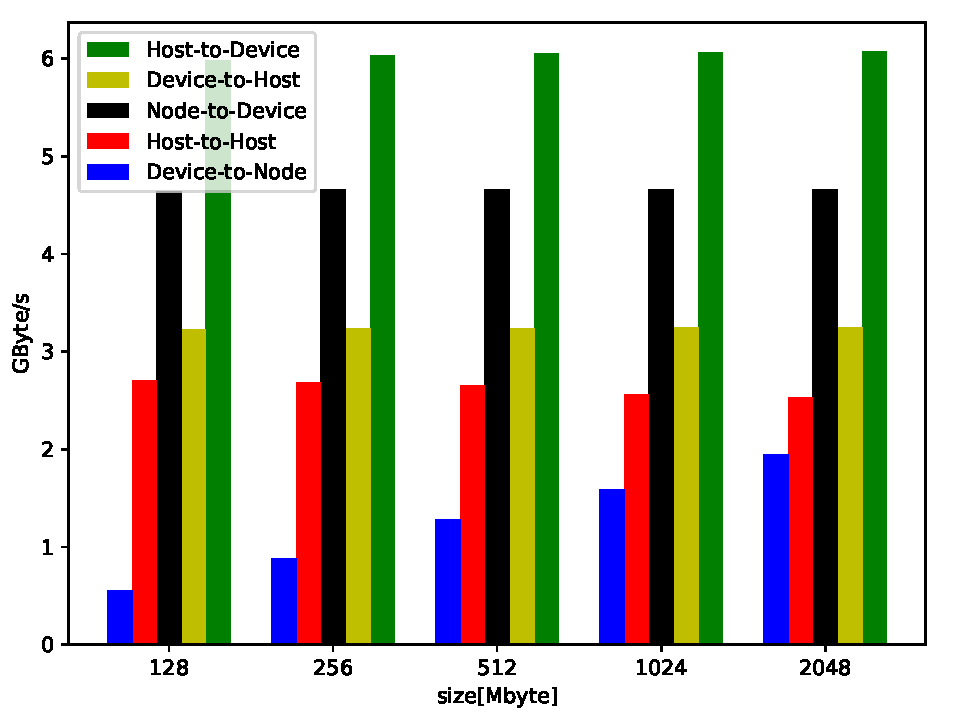
\includegraphics[width=\textwidth]{bw-plot}
	\end{minipage}\hfill
	\begin{minipage}{0.5\textwidth}
		\centering
		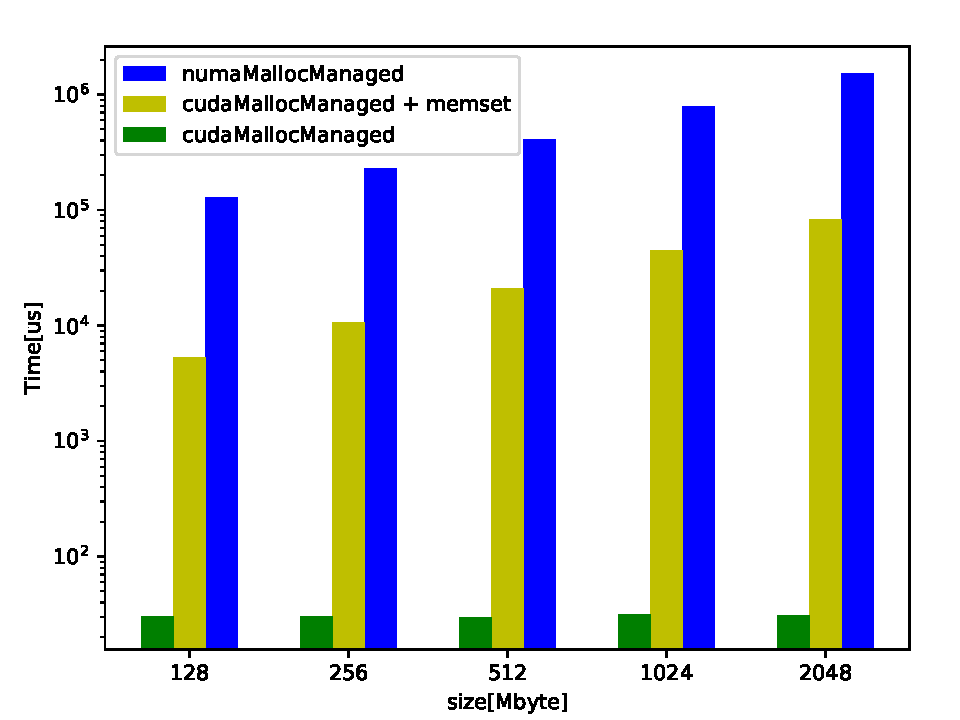
\includegraphics[width=\textwidth]{alloc-plot}
	\end{minipage}
	\caption{(L): Bandwidths achieved with the NUMA interface \newline (R): Allocation time compared between NUMA interface and CUDA interface}
	\label{f:micro}
\end{figure}
\subsection{Memory Migration}
Moving data inside the system can be the defining factor for the performance of an application. A series
of benchmarks quantifies the impact of data migration between different NUMA nodes and CUDA devices.

Figure \ref{f:micro} shows bandwidth measurements for data sets of various sizes. Both Host-to-Device and Device-to-Host
match the bandwidths achieved with CUDA (not displayed here). This means the wrapper does not reduce the performance
of already existing functionality.
Node-to-Device shows the bandwidth for transfers from NUMA nodes that are not directly connected to the device.

Host-to-host performance displays the achievable transfer bandwidth between two NUMA nodes and is depending on the used interconnect and the available memory bandwidth. The constant
performance shows that overheads caused by thread starting and joining can be neglected.

The Device-to-Node transfer shows the achievable bandwidth when copying data from a device to another NUMA node.
The achievable bandwidth is lower than a normal device-to-host transfer because twice the data needs to be moved, first
from device to the host, then to the targeted NUMA node.


\subsection{Memory Footprint}
Since memory is allocated for every NUMA node on the system, the memory footprints is multiplied by the number of NUMA nodes
in the system. The memory footprint is increased the factor that is the number of NUMA nodes in the system. 

\section{Application Benchmark}
To measure NUMA effects on an application, this benchmark runs a heterogeneous  pseudo-workload that quantifies the effects of NUMA locality for workloads that are shared between host and device. The workload performs an increment on every data element and ensures data movements are not optimized out by compilers
or the runtime and to simulate work that is performed during CPU and GPU computations.
First the benchmark performs the workload on one GPU and the NUMA node with the closest proximity. This ideal placing
serves as a reference for later runs. 
To measure the NUMA effects, the same workload is executed on the second GPU, with varying NUMA nodes. Which NUMA node the data is placed on, can be configured. This is used to measure how expensive non-optimal NUMA placement can be.

Performance is evaluated by relative increase of total execution time between first (ideal) and second run. 
The increase is the time lost due to data movement across NUMA nodes. Total time of second run includes
the time required to migrate the data to another NUMA node, if migration is performed.

Figure \ref{f:appaff} displays how performance is affected by multiple factors, for workloads that use
explicit prefetching of data between host and device.
\begin{itemize}
	\item \textbf{Size:} Size of workload.  
	\item \textbf{Kernel Runtime:} How long a single computation is performed. This is controlled by the number of workload iterations. Applied separately to CPU and GPU kernel.
	\item \textbf{Iterations:} How often CPU and GPU take turns in the computation. Increasing the parameter increases the number of times data is moved between host and device.
	\item \textbf{Affinity:} Control if data is moved to the NUMA node with the PCIe controller of the second GPU.
\end{itemize}

Generally the data in Figure \ref{f:appaff} suggest that every factor that contributes to an increased
computation runtime  mitigates the influence of NUMA migration on overall execution time, which is only depending on the size of the workload and available hardware. 

First we will look at the short running kernels (3 iterations of the workload). Here we see a spike
in the black bar for the workload of 128 MByte with no affinity and low data movement. The reason for this spike is the lower bandwidth and higher latency between host and device memory, which weigh in heavy against the very short
overall runtime. 

Since more application iterations also mean a higher compute time (3*3 iterations vs. 3*16 iterations) the effects are less visible. The blue bars dominate larger workloads because of the high
amount of traffic between host and device which is impaired by NUMA effects and small compute time in-between.

The green bar shows the best performance because it only hast to perform one Node-to-Node copy
and afterwards can benefit from the full bandwidth available between host and device. So the visible runtime increase is almost exclusive
the cost of one Node-to-Node transfer. For the yellow bar this static overhead of one data migration is larger due to a lower overall computation time, explaining the higher increase in runtime.

\begin{figure}
	\centering
	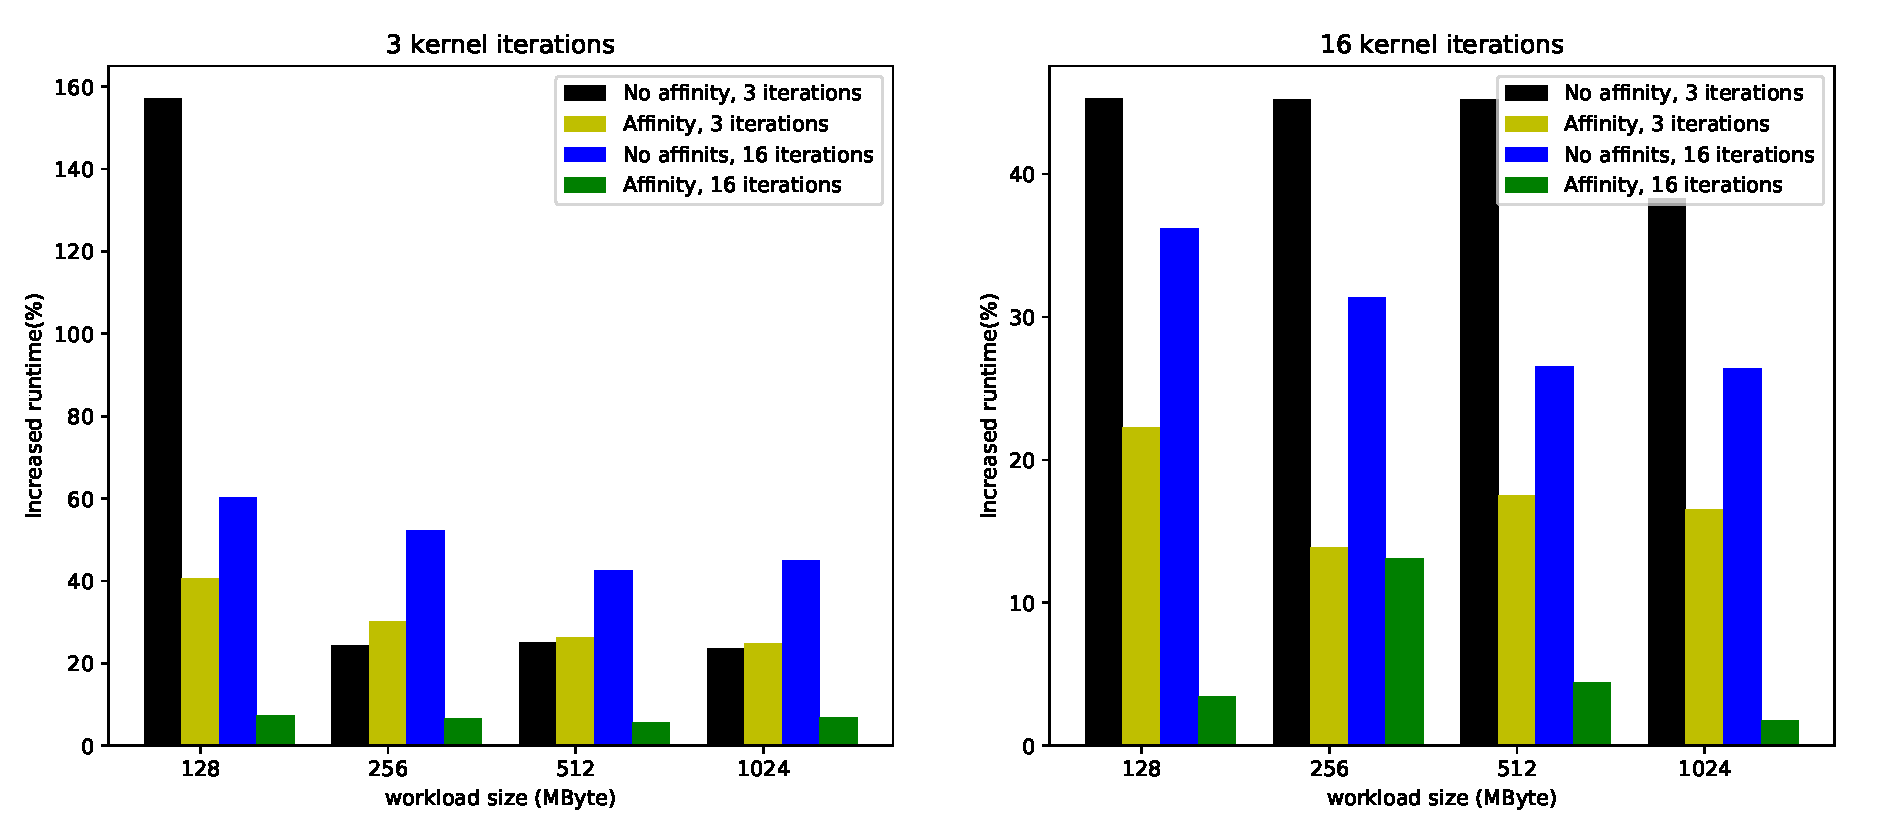
\includegraphics[width=\textwidth]{app-affinity}
	\caption{ NUMA-Effects on pseudo-workload. Displayed as increase of runtime relative to a run with ideal NUMA placement between host and device. With explicit data movement.
		The left hand side shows the relative increase in short running computational kernels.
		The right hand side shows the retlative increase on long computational kernels.}
	\label{f:appaff}
\end{figure}

\begin{figure}
	\centering
	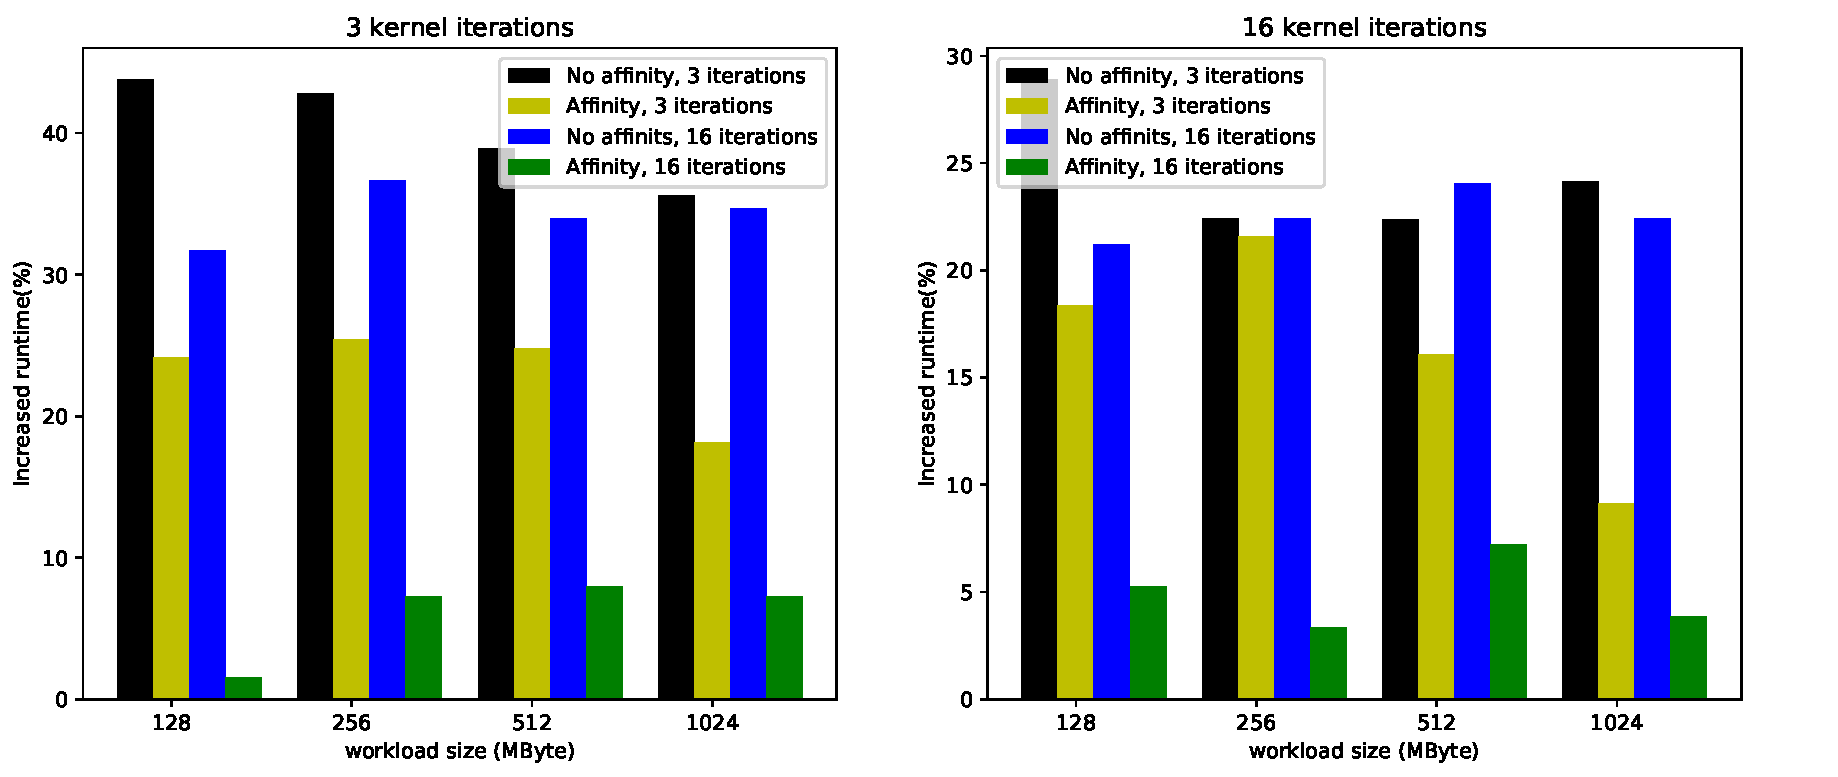
\includegraphics[width=\textwidth]{app-perf}
	\caption{ NUMA-Effects on pseudo-workload. Displayed as increase of runtime relative to a run with ideal NUMA placement between host and device. With implicit data movement.
		The left hand side shows the relative increase in short running computational kernels.
The right hand side shows the retlative increase on long computational kernels.}
	\label{f:apppref}
\end{figure}
For longer running kernels (16 kernel iterations) the data movement becomes less significant compared to compute time. Thus, the effects of NUMA locality are less visible in the data and the relative
performance overhead is reduced for all configurations, except the green one. It remains on its already
low level of overhead.

Figure\ref{f:apppref} shows the same experiment, but in this experiment data movement between host and device happend implicitly, using page-faults. The results show that the general assumptions about the data in \ref{f:appaff} still
hold true, however to smaller extend. This means that implicit data-movement creates a larger overhead, 
making NUMA effects less visible. In return this means that the explicit data movement benefits the overall
performance.
\begin{figure}
	\centering
	\begin{tabular}{|r|r|r|r|r|r|}
		\hline 
		Size [MByte] & Iterations & Kernel It. & Reference & Affinity & No Affinity\\ 
			\hline 
	128 & 3 & 3 & 251.25 & 353 & 636.5 \\ 
	\hline 
	128 & 3 & 16 &1328.75  & 1426 & 1936 \\ 
	\hline 
	128 & 16 & 3 & 429.5 & 525.25 & 584.25 \\ 
	\hline 
	128 & 16 & 16 & 2275.75 & 2354.5 & 2923.75 \\ 
	\hline 
	256 & 3 & 3 & 498.25 & 648.75 &  750.75\\ 
	\hline 
	256 & 3 & 16 & 2632 &2809.25  & 3801.5 \\ 
	\hline 
	256 & 16 & 3 & 876.5 & 998 & 1105.75 \\ 
	\hline 
	256 & 16 & 16 & 4367.25 & 4938.25 &5533.25  \\ 
	\hline 
	512 & 3 & 3 & 994 & 998 & 1429.75  \\ 
	\hline 
	512 & 3 & 16 & 5282.5 & 5583 & 7621 \\ 
	\hline 
	512 & 16 & 3 & 1701.25 & 1998.75 & 2172 \\ 
	\hline 
	512 & 16 & 16 & 8845 & 9237 & 10977.8 \\ 
	\hline 
	1024 & 3 & 3 &1958.25  & 2443.75  &2883.75 \\ 
	\hline 
	1024 & 3 & 16 & 10337 & 11054.8 &14645.5 \\ 
	\hline 
	1024 & 16 & 3 & 3336.5 & 3887.5 & 4292.25\\ 
	\hline 
	1024 & 16 & 16 & 17759.5  & 18078.2 & 22268.5\\ 
	\hline
	\end{tabular} 
	\label{tab:pref}
	\caption{Absolute Runtimes with Prefetch.}
\end{figure}
\begin{figure}
	\centering
	\begin{tabular}{|r|r|r|r|r|r|}
		\hline 
		Size [MByte] & Iterations & Kernel It. & Reference &  Affinity & No Affinity \\ 
		\hline 
	128 & 3 & 3 & 359.75 & 446.5 & 499.75 \\ 
	\hline 
	128 & 3 & 16 & 1918.5 & 1948.5 & 2507.75  \\ 
	\hline 
	128 & 16 & 3 & 534 & 632 & 683.25 \\ 
	\hline 
	128 & 16 & 16 & 2879.25 & 3031.25 & 3461 \\ 
	\hline 
	256 & 3 & 3 & 686 & 860.25 & 969 \\ 
	\hline 
	256 & 3 & 16 & 3684.5 & 3952.25 & 4939 \\ 
	\hline 
	256 & 16 & 3 & 1035.25 & 1258.75 & 1301.75 \\ 
	\hline 
	256 & 16 & 16 & 5584.5 & 5772.5 & 6606.25 \\ 
	\hline 
	512 & 3 & 3 & 1364 & 1702 & 1884.5 \\ 
	\hline 
	512 & 3 & 16 & 7209.25 & 7783 & 9883.5 \\ 
	\hline 
	512 & 16 & 3 & 2064.5 & 2396.5 & 2536.75  \\ 
	\hline 
	512 & 16 & 16 & 10868.2 & 11655 & 13499.5 \\ 
	\hline 
	1024 & 3 & 3 &2845.25  & 3361.75 &3693 \\ 
	\hline 
	1024 & 3 & 16 & 14395 & 15439 &19315 \\ 
	\hline 
	1024 & 16 & 3 & 4254 & 4641.5 & 5089\\ 
	\hline 
	1024 & 16 & 16 & 21778 & 22614.2 &26411.8 \\ 
	\hline
	\end{tabular}
	\label{tab:npref}
		\caption{Absolute Runtimes without Prefetch}
\end{figure}
	\chapter{Conclusions}\label{c:conc}
Extending CUDA's unified memory with NUMA locality features proved to be difficult due to restrictions by CUDA and the Linux 
kernel. Memory advices for implicit data movement can not be replicated in the Linux memory system. Replicating the
explicit data movement was also not trivial, because first-touch allocation is required and at the same time not 
possible during execution.

To work around the restrictions of both, Linux and Nvidia, inefficiencies are introduced that could prove 
critical for real world applications, especially the inefficient memory allocation and increased memory
footprint. Resolving these issues would require new functionalities implemented by the vendors, for example, the option that
unified memory can be allocated on the host side first. The data transfer from device to host would be eliminated and
first-touch binding would be more efficient. Also, allowing certain API-calls from inside a stream callback function, especially memory
(de-)allocation, would lead to a normalized memory footprint that is only increased during the migration.

Despite these difficulties,  the data from micro- and application benchmarks 
show that NUMA awareness in CUDA applications can have a big influence on the performance, 
depends on factors like size of workload, kernel runtime and 
intensity of data movement between host and device. 


\section{Future Work}
To continue this project in the future and making it more applicable for real-world applications the following
points should be addressed. (1) Making it platform independent. Parts of the code required for memory allocation is currently Linux specific. (2) Reducing the memory footprint. While an ideal
solution would require action by the vendor, in the current version some kind of garbage collector could
be implemented, which deletes buffers that are marked as trash by the callback function. This would allow allocation of memory
on demand before the callback is added to the stream and deleting the old data at a later point in execution, but before all the data is freed.
%	\newpage
%\newglossaryentry{query}{
%	name={Query},
%	description={
%		Suchanfrage, meist in einer speziellen Syntax. Enth�lt Informationen �ber die Suche und die Angeforderten Werte
%	}		
%}

% Roman pagination for listing, continuing from ToC 
%\pagenumbering{Roman}
%\setcounter{page}{3}
%\printindex
%\glsaddall
%\printglossaries
%\lstlistoflistings\newpage
%\listoffigures\newpage
%\listofmyequations\newpage
%\singlespacing
\bibliographystyle{ieeetr}
\bibliography{report}
\end{document}
